% !TEX root = ../main.tex

\section{SPI Signal Integrity}
\label{sec:results-spi}

\scaffold{
  \textbf{Paragraph 1, timing and content.} Captures of SPI0 at TP5--TP9 show a clock of \qty{3.95}{\mega\hertz} (the system clock of \qty{150}{\mega\hertz} divided by 38 for the requested \qty{4}{\mega\hertz}), SPI mode~0, and chip-select guards of \qty{9.8}{\micro\second} and \qty{11.45}{\micro\second} for the configured \qty{10}{\micro\second}. One data-register read takes \qty{30.65}{\micro\second} with the chip selected, of which \qty{9.4}{\micro\second} is clocking; decoding the bits gives the read command \code{0x44} followed by a 24-bit result. State that the guards dominate a transaction but are negligible against the \qty{4}{\milli\second} conversion time of a reading.
}

\scaffold{
  \textbf{Paragraph 2, edges.} \Cref{fig:spi-edges} shows clock and data edges captured at 10X: rise times of \qty{10.2}{\nano\second} (clock) and \qty{11.2}{\nano\second} (data), fall time \qty{8.4}{\nano\second}, overshoot within one oscilloscope step (\qty{40}{\milli\volt}), no ringing. The data line changes on the falling clock edge and is sampled on the rising one, so it is stable for about \qty{127}{\nano\second} on either side; a \qty{10}{\nano\second} edge uses about \qty{8}{\percent} of the half period. The edges are slowed on purpose by the \qty{47}{\ohm} series resistors. Two notes for honesty: the first capture at 1X showed edges of 24 to \qty{27}{\nano\second}, which was the probe's load; and the 10X capture was averaged, which supports \enquote{no ringing} but says nothing about one-off glitches.
}

\begin{figure}[htbp]
  \centering
  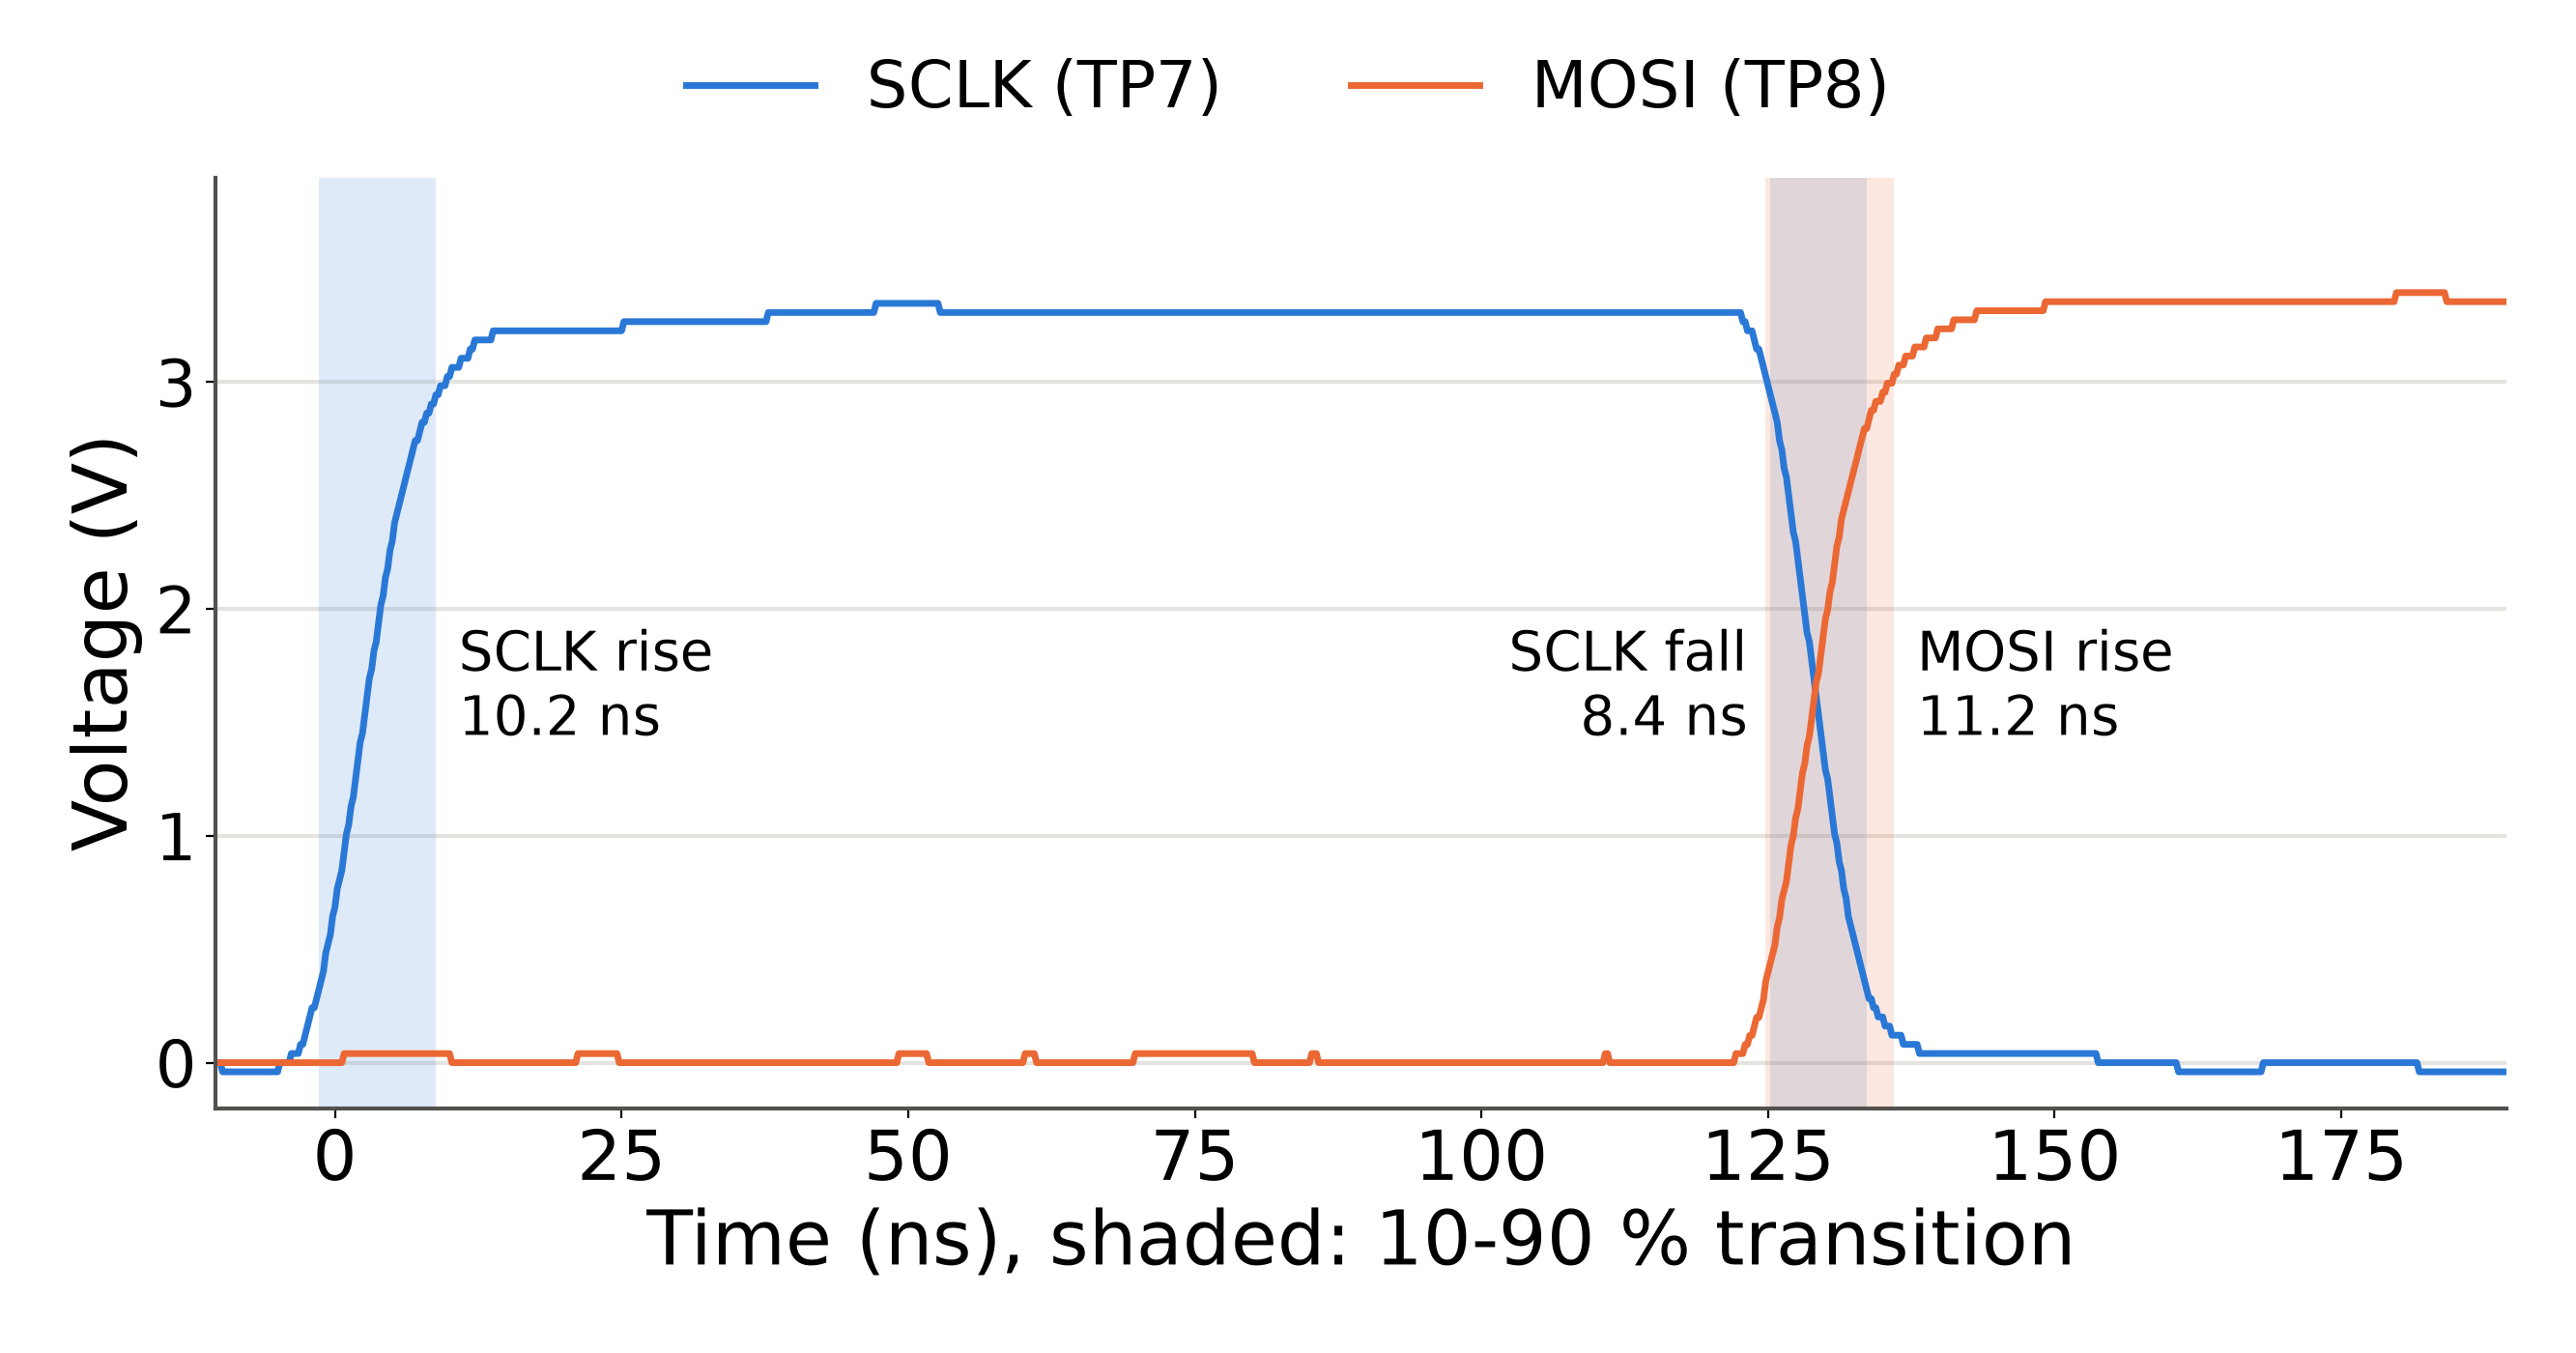
\includegraphics[width=0.85\linewidth]{05-results/figures/spi-edges}
  \titledcaption{SPI Edges}{\scaffoldinline{State conditions (10X probes, SCLK at TP7, MOSI at TP8, averaged capture) and that the shaded bands are the 10 to \qty{90}{\percent} transitions with their durations. Source: \code{measurements/create\_plots.py}, data \code{spi\_edges\_rise.csv}.}}
  \label{fig:spi-edges}
\end{figure}

\scaffold{
  \textbf{Paragraph 3, error-free transfer.} Firmware-side check: at \qty{4}{\mega\hertz} with a \qty{10}{\micro\second} guard, 300 consecutive readings contained no outlying code (more than six robust standard deviations from the median), where the breadboard had produced flipped bits at \qty{4}{\mega\hertz} and needed \qty{50}{\micro\second}.
}
